\documentclass[11pt]{standalone}
\usepackage{amssymb}
\usepackage{amsmath}
\usepackage[no-math]{fontspec}
\usepackage{unicode-math}
\setmainfont{Libertinus Sans}
\setsansfont{Libertinus Sans}
\setmathfont{Libertinus Math}
\usepackage{pgf,xcolor}
\usepackage{tikz}
\usetikzlibrary{arrows.meta, backgrounds, calc}
\usepackage{pgfplots}
\pgfplotsset{compat=newest}
\usepackage{pifont}

\definecolor{my_darkgray}{HTML}{484949}
\definecolor{my_lightgray}{HTML}{F3F4F4}
\definecolor{my_darkblue}{HTML}{005A94}
\definecolor{my_lightblue}{HTML}{CCDEE9}
\definecolor{my_yellow}{HTML}{FFEC7F}
\definecolor{my_red}{HTML}{E60000}
\definecolor{my_orange}{HTML}{E87846}

\begin{document}
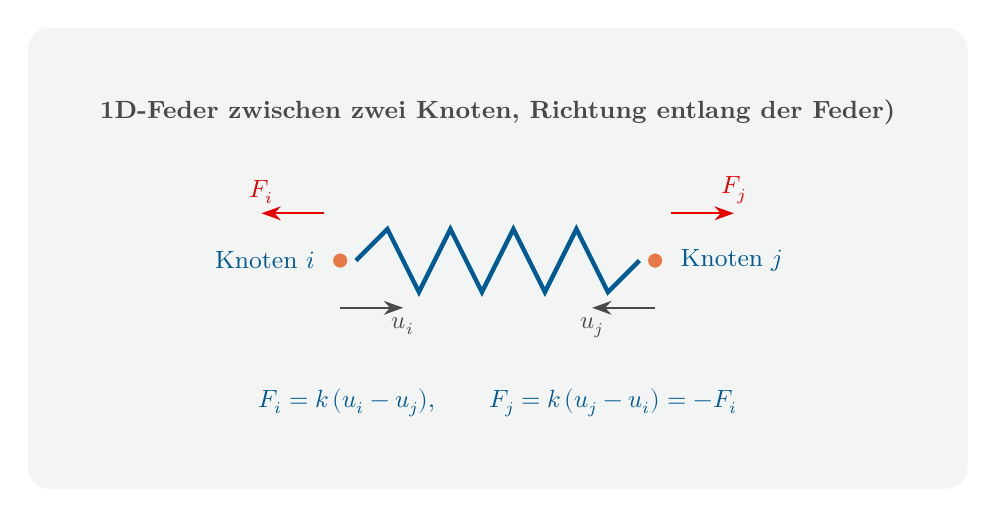
\begin{tikzpicture}[
    show background rectangle,
    background rectangle/.style={fill=my_lightgray, rounded corners=8pt},
    inner frame sep=0.8cm,
    annotation/.style={draw=my_darkgray, thick, -{Stealth[length=7pt, width=5pt]}}
]

    % Knotenpositionen (links: i, rechts: j)
    \coordinate (Ni) at (-2,0);
    \coordinate (Nj) at ( 2,0);

    % Knoten als Punkte
    \draw[fill=my_orange, draw=my_lightgray, thick] (Ni) circle (3pt);
    \draw[fill=my_orange, draw=my_lightgray, thick] (Nj) circle (3pt);

    % Knotenlabels links/rechts
    \node[font=\small, text=my_darkblue, anchor=east]
        at ($(Ni)+(-0.2,0)$) {Knoten $i$};
    \node[font=\small, text=my_darkblue, anchor=west]
        at ($(Nj)+(0.2,0)$) {Knoten $j$};

    % Feder als gezackte Linie zwischen den Knoten
    \draw[draw=my_darkblue, ultra thick]
        (-1.8,0) --
        (-1.4,0.4) --
        (-1.0,-0.4) --
        (-0.6,0.4) --
        (-0.2,-0.4) --
        (0.2,0.4) --
        (0.6,-0.4) --
        (1.0,0.4) --
        (1.4,-0.4) --
        (1.8,0);

    % Kräfte F_i und F_j entlang der Feder (1D-Richtung)
    \draw[annotation, draw=my_red]
        ($(Ni)+(-0.2,0.6)$) -- ($(Ni)+(-1.0,0.6)$);
    \node[font=\small, text=my_red, anchor=south]
        at ($(Ni)+(-1.0,0.6)$) {$F_i$};

    \draw[annotation, draw=my_red]
        ($(Nj)+(0.2,0.6)$) -- ($(Nj)+(1.0,0.6)$);
    \node[font=\small, text=my_red, anchor=south]
        at ($(Nj)+(1.0,0.6)$) {$F_j$};

    % Verschiebungen u_i und u_j entlang der Feder
    \draw[annotation]
        ($(Ni)+(0,-0.6)$) -- ($(Ni)+(0.8,-0.6)$);
    \node[font=\small, text=my_darkgray, anchor=north]
        at ($(Ni)+(0.8,-0.6)$) {$u_i$};

    \draw[annotation]
        ($(Nj)+(0,-0.6)$) -- ($(Nj)+(-0.8,-0.6)$);
    \node[font=\small, text=my_darkgray, anchor=north]
        at ($(Nj)+(-0.8,-0.6)$) {$u_j$};

    % Hooke-Gesetz als Text unterhalb der Feder
    \node[font=\small, text=my_darkblue, anchor=north] at (0,-1.5)
        {$F_i = k\,(u_i - u_j), \qquad F_j = k\,(u_j - u_i) = -F_i$};

    % Titel der Abbildung
    \node[font=\small\bfseries, text=my_darkgray, anchor=south] at (0,1.6)
        {1D-Feder zwischen zwei Knoten, Richtung entlang der Feder)};

\end{tikzpicture}
\end{document}